% !TEX root = ../master-thesis.tex

% \textbf{Introduction and motivation.}
Manipulating the internal spin state of ultracold atoms is essential for deterministic state preparation and spin-resolved imaging in quantum simulation experiments. Two primary methods for controlled spin transitions are Landau-Zener (LZ) sweeps and resonant $\pi$-pulses. LZ transitions involve adiabatically sweeping across a spin resonance and offer robustness against parameter fluctuations, while $\pi$-pulses provide faster operation but require precise calibration of pulse parameters. In this experiment, spin manipulation serves two functions: flipping atoms to stretched states for efficient spin-resolved imaging, and selective removal of specific spin states during state preparation. The choice between LZ and $\pi$-pulse methods depends on the specific transition and its sensitivity to experimental noise.

% \textbf{Landau-Zener transition.}
The Landau-Zener transition describes non-adiabatic transitions between quantum states when their energy separation varies linearly in time. The governing Hamiltonian is:
\begin{equation*}
H_{\text{LZ}}(t) = \frac{\hbar}{2}
\begin{pmatrix}
\Delta(t) & \Omega \\
\Omega & -\Delta(t)
\end{pmatrix},
\label{eq:LZ_Hamiltonian}
\end{equation*}
where $\Delta(t) = \alpha t$ is the time-dependent detuning and $\Omega$ is the coupling strength. The transition probability is given by:
\begin{equation*}
P_{\text{LZ}} = 1 - \exp\left(-\frac{\pi \Omega^2}{2\alpha}\right).
\label{eq:LZ_probability}
\end{equation*}
For slow sweeps ($\alpha \ll \Omega^2$), near-complete transitions are achieved. The method's robustness against magnetic field fluctuations makes it suitable for transitions sensitive to experimental noise.

% \textbf{Rabi $\pi$-pulse.}
The $\pi$-pulse method uses resonant driving to achieve rapid population transfer. Under resonant conditions ($\Delta=0$), a pulse duration $t_\pi = \pi/\Omega$ results in complete spin inversion. The fidelity depends on detuning accuracy:
\begin{equation*}
P_{\pi} = \frac{\Omega^2}{\Omega^2+\delta^2}\sin^2\left(\frac{\sqrt{\Omega^2+\delta^2}}{2}t_{\pi}\right),
\label{eq:pi_fidelity}
\end{equation*}
where $\delta$ is the detuning. This method offers faster operation but requires stable experimental conditions.

\begin{figure}
    \centering
    \addletter{105}{a}
    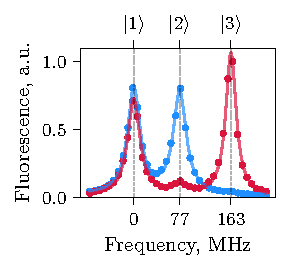
\includegraphics{fig-py/spin-flip-1.pdf}  \phantom{4}
    \addletter{105}{b}
    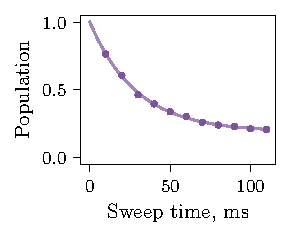
\includegraphics{fig-py/spin-flip-2.pdf}  \phantom{4}
    \addletter{105}{c}
    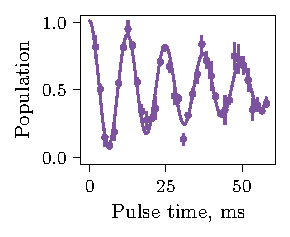
\includegraphics{fig-py/spin-flip-3.pdf}  \phantom{4}
    \caption[Characterization of spin manipulation protocols]{
        \textbf{Characterization of spin manipulation protocols.}
        (a) Fluorescence signal before (blue) and after (red) Landau-Zener sweep between states $\ket{2}$ and $\ket{3}$. 
        (b) Final population in $\ket{2}$ versus sweep duration, consistent with Landau-Zener model. 
        (c) Rabi oscillations for resonant RF $\pi$-pulse between states $\ket{2}$ and $\ket{3}$.
    }
    \label{fig:spin-flip}
\end{figure}

% \textbf{Implementation in this experiment.}
The current experimental setup employs both methods optimized for different transitions. For the RF transition $\ket{2} \to \ket{3}$, $\pi$-pulses are used with a Rabi frequency of 35~kHz, achieving 99\% fidelity. For the MW transition $\ket{1} \to \ket{6}$, Landau-Zener sweeps are preferred due to the larger differential magnetic moment that makes this transition more sensitive to magnetic field noise. Operating at 75~kHz coupling strength, LZ sweeps achieve 95\% fidelity while maintaining robustness against parameter fluctuations.
Spin-state populations are measured by frequency scanning while recording fluorescence signals from atoms in the ODT or optical tweezers, as demonstrated in Fig.~\ref{fig:spin-flip}a.